\section{5G Data Plane \label{sec:5GDataPlane}}
5G technology aims to satisfy the increasing requirements of the customers of mobile service 
in terms of higher throughput and lower processing latency. 
The major difference in  the processing of data and signalling packets between 5G and earlier standards is control-user plane 
separation and the use of network function virtualization. Forwarding of packets, 
authentication of mobile devices, session establishment and management  are some of the network functions required in the core of a telecommunication network. 
These network functions run on different or same physical machines as 
virtual machines for easier migration/scaling. 
\begin{figure}[htbp]
	\centering
       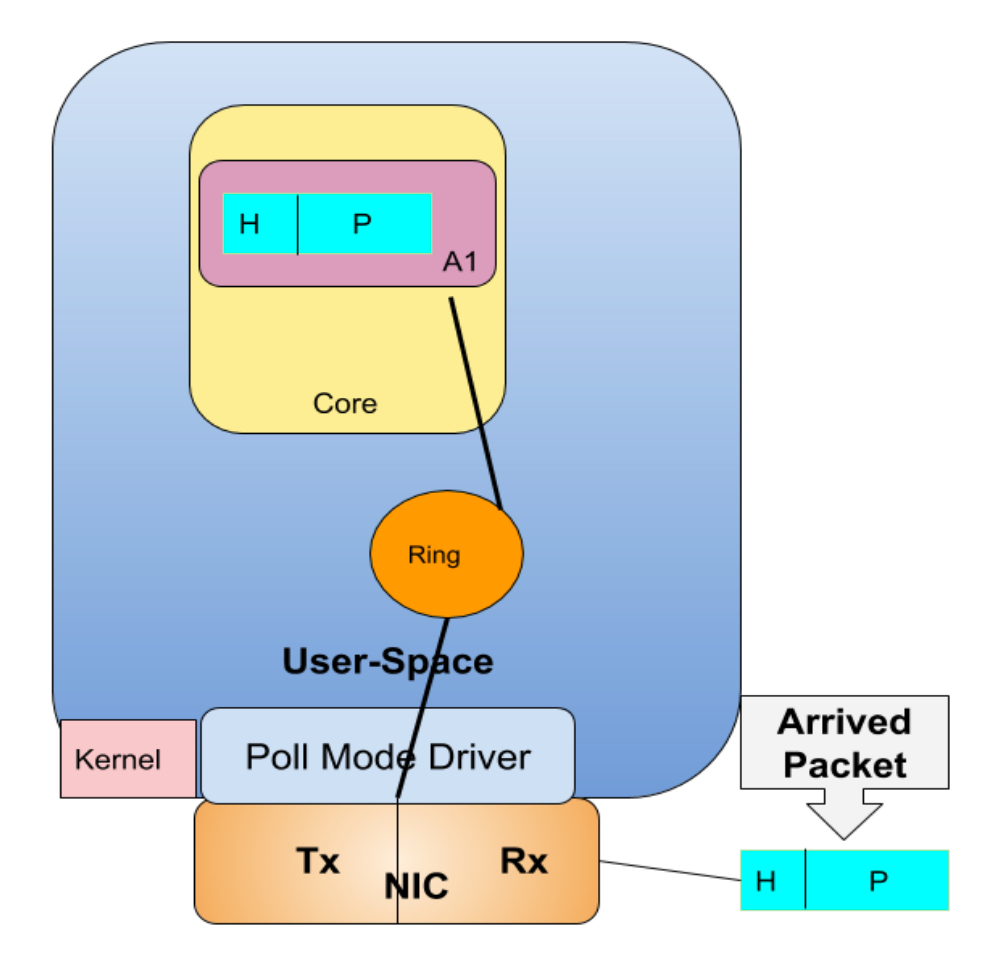
\includegraphics[width=0.7\textwidth]{fig/dpdkOverview.png}
       %  \setlength{\abovecaptionskip}{-2pt}
       \setlength{\belowcaptionskip}{-12pt}
	\caption{DPDK kernel bypass}
	\label{fig:dpdkOverview}
       \end{figure}

This project is mainly concerned with the data forwarding plane. The network functions in our setup run as separate processes.
The high speed data plane is required to meet the ever increasing demands of higher bandwidth and lower latency. The Linux kernel stack cannot meet this demand as it is a general purpose stack catering to different protocols and there is a packet copy overhead from kernel space to the user space for reading the packet payload. The technqiues used to overcome this limitation of the Linux stack is the use of kernel bypass frameworks like Data Plane Development Kit (DPDK) \cite{dpdk}, and the use of programmable NICs to offload processing functions in the hardware. 
DPDK runs in software and there is a single copy of packets from NIC buffer to the
 user space. DPDK libraries are optimized for high speed data processing. The use
  of superpages, lockless data structures, better memory management and customized device drivers for
   various NICs are among some of the salient features of DPDK framework which
   enables high speed processing of data. 
\begin{figure}[htbp]
	\centering
       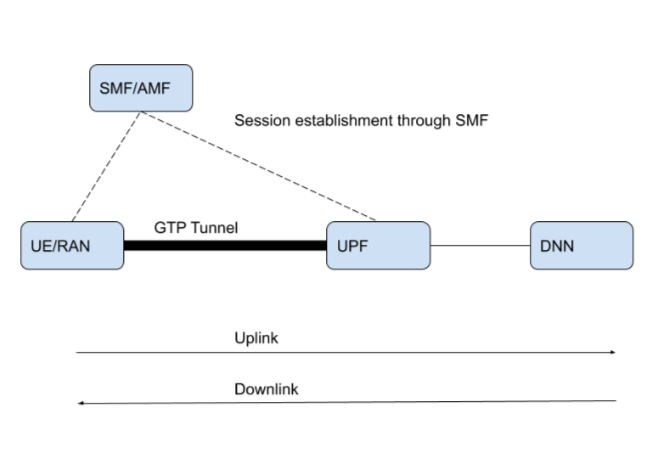
\includegraphics[width=0.7\textwidth]{fig/5Goverview.png}
       %  \setlength{\abovecaptionskip}{-2pt}
       \setlength{\belowcaptionskip}{-12pt}
	\caption{5G Forwarding Plane.}
	\label{fig:5gForwardingPlane}
       \end{figure}



   The main network functions in the data plane are 
   \begin{itemize}
	   \item \textbf{Radio Access Network (RAN)} RAN is the main point of contact for all the user equipments and is an entry point to Non Access Stratum in the 5G network.
	   \item \textbf{User Plane Function (UPF)}
	   UPF is responsible for forwarding the incoming packets from the RAN to the public internet. UPF ensures QoS guarantees, collects usage statistics useful for charging purpose, buffers packets (if required).
	   
	   \item \textbf{Data Network Name}
	   DNN is the gateway to the public internet. DNN forwards the uplink packets from UEs to the public internet and all the incoming packets for the UEs (downlink) are received at the DNN.
   \end{itemize}
  
\section{Problem Statement}
\begin{itemize}
	\item \textbf{User Plane Function: Implement the packet steering offload  mechanism in the UPF.} 
	
	The packets coming from RAN are tunneled in the application layer of an outer 
	packet.The tunneled application level header  contains the information 
	associating the data packet to a corresponding user. The outer IP/UDP headers
 	are same for all the packets between a set of network functions. The key for
	the standard hash computation in the hardware  are the outer packet headers.
	The goal here is to implement the UPF design in which the packets are
	redirected in the hardware to the multiple cores for parallel processing
	based on the inner packet and application level headers. The redirection based on inner packet fields ensure that packets of the same flow are directed to the same core resulting in better spatial locality.
	\item \textbf{Radio Access Network}  Extend the existing DPDK based RAN by adding new features and refactor, clean the code to make RAN extensible in the future.  The new features are aimed at emulating the real-time traffic and to benchmark various designs of UPF.  
\end{itemize}

\section{Major Contributions}
\begin{itemize}
	\item The UPF design which with the hardware based redirection on the inner packet headers was implemented. 
	\item Two new features were added in the RAN - measurement of control plane latency and simultaneous transfer of control plane and the data plane traffic.
	\item The source code of the existing RAN was entirely refactored and restructured.
	\item Conducted experiments for benchmarking different models of the UPF for measurement of throughput and latency metrics under different load conditions.
\end{itemize}
